\section{Моделирование предметной области и разработка требований}
\label{sec:func}
 
\subsection{Разработка функциональной модели предметной области}
Диаграмма вариантов использования (сценариев поведения, прецедентов) является исходным концептуальным представлением системы в процессе ее проектирования и разработки. Данная диаграмма состоит из актеров, вариантов использования и отношений между ними. При построении диаграммы могут использоваться также общие элементы нотации: примечания и механизмы расширения.
Суть данной диаграммы состоит в следующем: проектируемая система представляется в виде множества актеров, взаимодействующих с системой с помощью так называемых вариантов использования. При этом актером (действующим лицом, актантом, актором) называется любой объект, субъект или система, взаимодействующая с моделируемой системой извне. В свою очередь вариант использования – это спецификация сервисов (функций), которые система предоставляет актеру. Другими словами, каждый вариант использования определяет некоторый набор действий, совершаемых системой при взаимодействии с актером. При этом в модели никак не отражается то, каким образом будет реализован этот набор действий.
Диаграмма вариантов использования ПС визуального анализа информации представлена на рисунке 3.1.
Зачастую в рамках разрабатываемой системы выделяют определённые роли пользователей, обладающие разными категориями прав. Каждая роль пользователей на диаграмме вариантов использования отображается отдельным действующим лицом.

В приложении существуют два действующих лица:
\begin{itemize}
  \item гость~-- незарегестрированный пользователь;
  \item пользователь~-- зарегестрированный пользователь, получивший доступ ко всему приложению.
\end{itemize}

\begin{figure}[H]
 \centering
   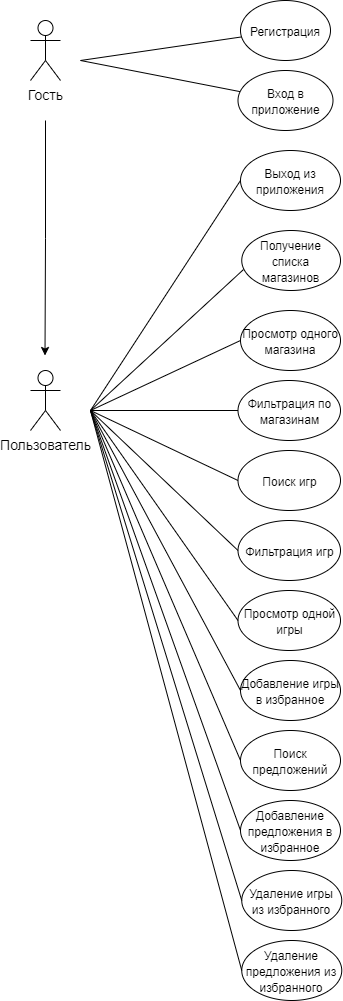
\includegraphics[scale=0.5]{use_case_diagram.png} 
   \caption{Диаграмма используемого программного средства}
   \label{fig:domain:use_case_diagram}
\end{figure}


\undersection{Регистрация}~\par

Регистрация гостя в приложении. Регистрация проходит через сторонний сервис Firebase Auth.

Основной сценарий:

\begin{itemize}
  \item гость нажимает на кнопку «Register»;
  \item гость вводит логин и пароль;
  \item если введенные данные верны, то пользователь регистрируется в приложении входит в систему;
  \item если данные неверны, пользователю показывается ошибка о неправильности данных;
  \item переход к началу сценария.
\end{itemize}

\undersection{Вход в приложение}~\par

Вход гостя в приложение. Вход проходит через сторонний сервис Firebase Auth.

Основной сценарий:

\begin{itemize}
  \item приложение запрашивает логин и пароль;
  \item гость вводит логин и пароль;
  \item если введенные данные верны, то пользователь входит в приложение;
  \item если данные неверны, пользователю показывается ошибка о неправильных данных;
  \item переход к началу сценария.
\end{itemize}

\undersection{Выход из приложения}~\par

Выход пользователя из приложения. Выход проходит через сторонний сервис Firebase Auth.

\begin{itemize}
  \item гость нажимает на кнопку «Sign Out»;
  \item гость выходит из приложения на экран регистрации.
\end{itemize}

\undersection{Получение списка магазинов}~\par

Получение пользователем списка магазинов на экран. Получение проходит через стороннее API по получению информации о магазинах.

\begin{itemize}
  \item пользователь нажимает на кнопку «Stores»;
  \item пользователь делает HTTP запрос на получение списка магазинов;
  \item приложение позволяет пользователю просмотреть весь список доступных магазинов.
\end{itemize}


\undersection{Просмотр одного магазина}~\par

Просмотр одного магазина. Получение проходит через стороннее API по получению информации о магазинах.

\begin{itemize}
  \item пользователь нажимает на кнопку «Stores»;
  \item пользователь делает HTTP запрос на получение списка магазинов;
  \item приложение позволяет пользователю просмотреть весь список доступных магазинов;
  \item пользователь нажимает на один из магазинов;
  \item пользователь делает HTTP запрос на получение дополнительной информации о магазине;
  \item приложение позволяет пользователю просмотреть дополнительную информацию о магазине (предложения и скидки магазина, описание, возможность перехода на просмотр информации о предложениях).
\end{itemize}

\undersection{Фильтрация по магазинам}~\par

Пользователь может совершать фильтрацию по магазинам во всем приложении. Можно включать и отключать различные магазины для поиска. Фильтрация происходит через стороннее API.

Первое использование:

\begin{itemize}
  \item пользователь нажимает на кнопку «Stores»;
  \item пользователь делает HTTP запрос на получение списка магазинов;
  \item приложение позволяет пользователю просмотреть весь список доступных магазинов;
  \item пользователь выключает один магазин нажатием на «галочку»;
  \item приложение запоминает выбор пользователя;
  \item приложение позволяет больше не фильтрует по этому магазину данные выдаваемые пользователю.
\end{itemize}

Второе использование:

\begin{itemize}
  \item пользователь нажимает на кнопку «Stores»;
  \item пользователь делает HTTP запрос на получение списка магазинов;
  \item приложение позволяет пользователю просмотреть весь список доступных магазинов;
  \item пользователь включает один магазин нажатием на «галочкой»;
  \item приложение запоминает выбор пользователя;
  \item приложение позволяет фильтрует по этому магазину данные выдаваемые пользователю.
\end{itemize}

\undersection{Поиск игр}~\par

Пользователь может совершать поиск по базе данных игр. Поиск происходит через стороннее API.

\begin{itemize}
  \item пользователь нажимает на кнопку «Search»;
  \item пользователь нажимает на вкладку «Games»;
  \item пользователь делает HTTP запрос на получение списка игр, дополняя его информацией о магазинах;
  \item приложение позволяет пользователю просмотреть весь список доступных игр;
  \item приложение позволяет пользователю задать в поисковой строке имя искомой игры;
  \item пользователь делает HTTP запрос на получение списка игр, но уже со значением поисковой строки;
  \item приложение позволяет пользователю просмотреть отфильтрованный список доступных игр по поисковой строке.
\end{itemize}

\undersection{Фильтрация игр}~\par

Пользователь может дополнительно фильтровать поиск по базе данных игр. Фильтрация поиска происходит через стороннее API.


\begin{itemize}
  \item пользователь нажимает на кнопку «Search»;
  \item пользователь нажимает на вкладку «Games»;
  \item пользователь делает HTTP запрос на получение списка игр;
  \item приложение позволяет пользователю просмотреть весь список доступных игр;
  \item приложение позволяет пользователю задать в поисковой строке имя искомой игры;
  \item пользователь нажимает на значок фильтрации и задает собственные критерии фильтрации (сортировка, рейтинг, наличие скидки);
  \item пользователь делает HTTP запрос на получение списка игр, но уже со значением поисковой строки;
  \item приложение позволяет пользователю просмотреть отфильтрованный список доступных игр по поисковой строке.
\end{itemize}

\undersection{Просмотр одной игры}~\par

Пользователь может просматривать дополнительную информацию об игре. Получение дополнительной информации об игре происходит через стороннее API.

\begin{itemize}
  \item пользователь нажимает на кнопку «Search»;
  \item пользователь нажимает на вкладку «Games»;
  \item пользователь делает HTTP запрос на получение списка игр;
  \item приложение позволяет пользователю просмотреть весь список доступных игр;
  \item пользователь нажимает на одну из игр;
  \item пользователь делает HTTP запрос на получение дополнительной информации об игре;
  \item приложение позволяет пользователю просмотреть дополнительную информацию об игре (описание, рейтинг, скидки в разных магазинах).
\end{itemize}


\undersection{Добавление игры в избранное}~\par

Пользователь может добавить игру в избранное. Добавление в избранное происходит локально с сохранением результата в Firebase.

\begin{itemize}
  \item пользователь нажимает на кнопку «Search»;
  \item пользователь нажимает на вкладку «Games»;
  \item пользователь делает HTTP запрос на получение списка игр;
  \item приложение позволяет пользователю просмотреть весь список доступных игр;
  \item пользователь нажимает на добавление в избранное одной из игр;
  \item пользователь делает HTTP запрос на добавление игры в избранное.
\end{itemize}

\undersection{Поиск предложений}~\par
Пользователь может совершать поиск по базе данных предложений. Поиск происходит через стороннее API.

\begin{itemize}
  \item пользователь нажимает на кнопку «Search»;
  \item пользователь нажимает на вкладку «Deals»;
  \item пользователь делает HTTP запрос на получение списка предложений;
  \item приложение позволяет пользователю просмотреть весь список доступных предложений;
  \item приложение позволяет пользователю задать в поисковой строке имя игры для которой будет совершаться поиск предложений;
  \item пользователь делает HTTP запрос на получение списка предложений, но уже со значением поисковой строки;
  \item приложение позволяет пользователю просмотреть отфильтрованный список доступных предложений по поисковой строке.
\end{itemize}


\undersection{Добавление предложения в избранное}~\par

Пользователь может добавить предложение в избранное. Добавление в избранное происходит локально с сохранением результата в Firebase.

\begin{itemize}
  \item пользователь нажимает на кнопку «Search»;
  \item пользователь нажимает на вкладку «Deals»;
  \item пользователь делает HTTP запрос на получение списка предложений;
  \item приложение позволяет пользователю просмотреть весь список доступных предложений;
  \item пользователь нажимает на добавление в избранное одного из предложений;
  \item пользователь делает HTTP запрос на добавление предложения в избранное.
\end{itemize}


\undersection{Удаление игры из избранного}~\par
Пользователь может удалить предложение из избранного. Удаление из избранного происходит локально с сохранением результата в Firebase.

\begin{itemize}
  \item пользователь нажимает на кнопку «Favorites»;
  \item пользователь нажимает на вкладку «Games»;
  \item пользователь делает HTTP запрос на получение списка избранных игр;
  \item приложение отображает пользователю список избранных игр;
  \item пользователь нажимает на удаление из избранного одной игры;
  \item пользователь делает HTTP запрос на удаление игры из избранного.
\end{itemize}



\undersection{Удаление предложения из избранного}~\par
Пользователь может удалить игру из избранного. Удаление из избранного происходит локально с сохранением результата в Firebase.

\begin{itemize}
  \item пользователь нажимает на кнопку «Favorites»;
  \item пользователь нажимает на вкладку «Deals»;
  \item пользователь делает HTTP запрос на получение списка избранных предложений;
  \item приложение позволяет пользователю просмотреть весь список избранных предложений;
  \item пользователь нажимает на удаление из избранного одного предложения;
  \item пользователь делает HTTP запрос на удаление предложения из избранного.
\end{itemize}

\subsection{Разработка функциональной модели предметной области}

Блок взаимодействия с незарегестрированными пользователями:

\begin{itemize}
    \item регистрация;
    \item ввод логина и пароля;
    \item вход в приложение.
\end{itemize}

Блок взаимодействия с зарегестрированными пользователями:

\begin{itemize}
    \item выход из приложения;
    \item получение списка магазинов с кэшированием локальную базу данных;
    \item просмотр одного магазина с кэшированием в локальную базу данных;
    \item фильтрация по магазинам;
    \item поиск игр;
    \item фильтрация игр;
    \item просмотр одной игры с кэшированием в локальную базу данных;
    \item добавление игры в избранное;
    \item поиск предложений;
    \item добавление предложения в избранное;
    \item удаление игры из избранного;
    \item удаление предложения из избранного.
\end{itemize}


\subsection{Логическая модель данных}

В последствии анализа сторонних API и функциональных требований к приложению была построения логическая модель данных в виде таблицы баз данных и их связей.

\begin{figure}[H]
 \centering
   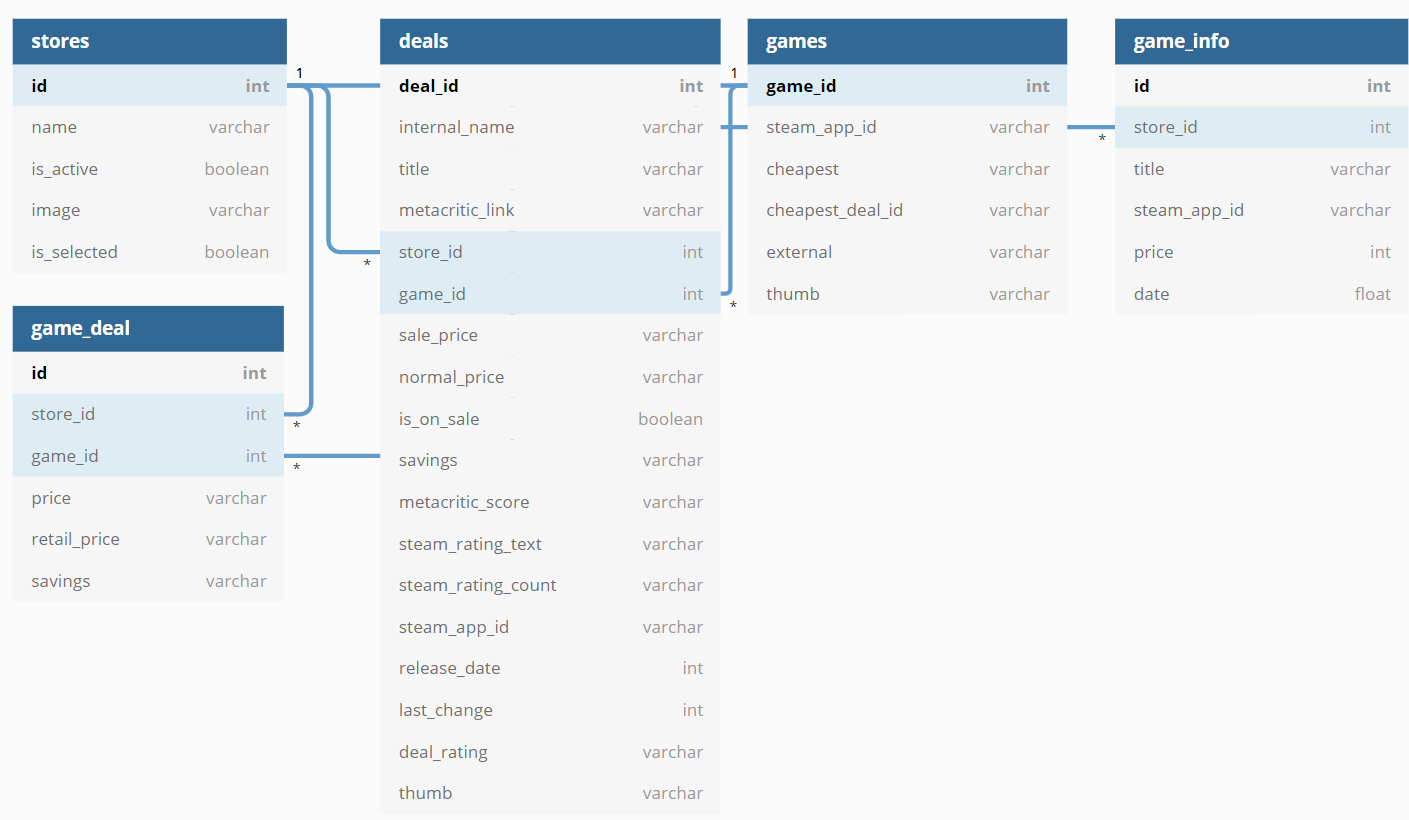
\includegraphics[scale=0.45]{logic_model.png} 
   \caption{Логическая модель}
   \label{fig:domain:logic_model}
\end{figure}

Таблица «Stores»~-- таблица магазинов полученных от сторонних API и интегрированных в приложение.~\par
\begin{table}[H]
\caption{Stores}
\label{table:func:stores}
 \centering
 \begin{tabular}
 {| >{\raggedright}m{0.02\textwidth}
 | >{\centering}m{0.3\textwidth}
 | >{\centering}m{0.18\textwidth}
 | >{\centering\arraybackslash}m{0.4\textwidth}|}
   \hline
   № & Имя & Тип & Описание \\
   \hline
   1 & 2 & 3 & 4 \\
 
   \hline
   1 & id & int & Идентификатор ключа \\
 
   \hline
   2 & name & varchar & Название магазина \\
 
   \hline
   3 & is\_active & boolean & Флаг активен ли магазин\\
 
   \hline
   4 & image & varchar & Ссылка на картинку \\

   \hline
   5 & is\_selected & boolean & Выбран ли магазин для фильтрации \\
 
   \hline
 \end{tabular}
\end{table}

Таблица «Deals»~-- таблица предложений полученных от сторонних API и интегрированных в приложение. ~\par
\begin{table}[H]
\caption{Deals}
\label{table:func:deals}
 \centering
 \begin{tabular}
 {| >{\raggedright}m{0.02\textwidth}
 | >{\centering}m{0.3\textwidth}
 | >{\centering}m{0.18\textwidth}
 | >{\centering\arraybackslash}m{0.4\textwidth}|}
   \hline
   № & Имя & Тип & Описание \\
   \hline
   1 & 2 & 3 & 4 \\
 
   \hline
   1 & deal\_id & int & Идентификатор ключа \\
   \hline
   2 & internal\_name & varchar & сокращенное название игры для приложения \\
   \hline
   3 & title & varchar & Название игры \\
   \hline
   4 & metacritic\_link & varchar & Ссылка на Metacritic \\
   \hline
   5 & store\_id & int & Внешний ключ модели магазина \\
   \hline
   5 & game\_id & int & Внешний ключ модели игры\\
   \hline
   6 & sale\_price & varchar & Цена игры на скидке\\
   \hline
   7 & normal\_price & varchar & Цена игры без скидки\\
   \hline
   8 & is\_on\_sale & boolean & На скидке ли игра\\
   \hline
   9 & savings & varchar & Теоритическая экономия\\
   \hline
   10 & metacritic\_score & varchar & Баллы Metacritic\\
   \hline
   11 & steam\_rating\_text & varchar & Описание рейтинга Steam\\
   \hline
   11 & steam\_rating\_count & varchar & Рейтинг Steam\\
   \hline
   12 & steam\_app\_id & varchar & Идентификатор в Steam\\
   \hline
   13 & release\_date & int & Дата выпуска\\
   \hline
   14 & last\_change & int & Дата последнего изменения\\
   \hline
   15 & deal\_rating & varchar & Рейтинг предложения\\
   \hline
   16 & thumb & varchar & Ссылка на картинку\\
   \hline
 \end{tabular}
\end{table}
Таблица «GameDeal»~-- таблица предложений по играм полученных в результате получения дополнительной информации о предложении.~\par
\begin{table}[H]
\caption{GameDeal}
\label{table:func:gamedeal}
 \centering
 \begin{tabular}
 {| >{\raggedright}m{0.02\textwidth}
 | >{\centering}m{0.3\textwidth}
 | >{\centering}m{0.18\textwidth}
 | >{\centering\arraybackslash}m{0.4\textwidth}|}
   \hline
   № & Имя & Тип & Описание\\
   \hline
   1 & 2 & 3 & 4\\
 
   \hline
   1 & id & int & Идентификатор ключа\\
 
   \hline
   2 & store\_id & int & Внешний ключ магазина\\

   \hline
   3 & game\_id & int & Внешний ключ игры\\

   \hline
   4 & price & varchar & Текущая цена\\
 
   \hline
   5 & retail\_price & varchar & Цена без скидки\\
 
   \hline
   6 & savings & varchar & Скидка\\
 
   \hline
 \end{tabular}
\end{table}
Таблица «Games»~-- таблица игр полученных от сторонних API и интегрированных в приложение.~\par
\begin{table}[H]
\caption{Games}
\label{table:func:games}
 \centering
 \begin{tabular}
 {| >{\raggedright}m{0.02\textwidth}
 | >{\centering}m{0.3\textwidth}
 | >{\centering}m{0.18\textwidth}
 | >{\centering\arraybackslash}m{0.4\textwidth}|}
   \hline
   № & Имя & Тип & Описание\\
   \hline
   1 & 2 & 3 & 4\\
 
   \hline
   1 & game\_id & int & Идентификатор ключа\\
 
   \hline
   2 & steam\_app\_id & varchar & Идентификатор в Steam\\

   \hline
   3 & cheapest & int & Самая низкая цена\\

   \hline
   4 & cheapest\_deal\_id & int & Внешний ключ предложения\\

   \hline
   5 & external & varchar & Ссылка на картинку в виде иконки\\
 
   \hline
   6 & thumb & varchar & Ссылка на картинку\\
 
   \hline
 \end{tabular}
\end{table}
Таблица «GameInfo»~-- таблица дополнительной информации об играх полученных в результате дополнительных запросов к сторонним API.~\par
\begin{table}[H]
\caption{GameInfo}
\label{table:func:gameinfo}
 \centering
 \begin{tabular}
 {| >{\raggedright}m{0.02\textwidth}
 | >{\centering}m{0.3\textwidth}
 | >{\centering}m{0.18\textwidth}
 | >{\centering\arraybackslash}m{0.4\textwidth}|}
   \hline
   № & Имя & Тип & Описание\\
   \hline
   1 & 2 & 3 & 4\\
 
   \hline
   1 & id & int & Идентификатор ключа\\

   \hline
   2 & store\_id & int & Внешний ключ магазина\\
 
   \hline
   3 & title & varchar & Название\\
   \hline
   4 & steam\_app\_id & varchar & Идентификатор в Steam\\
   \hline
   5 & price & int & Цена игры\\
   \hline
   6 & date & flaot & Дата выпуска\\
 
   \hline
 \end{tabular}
\end{table}


% Model — слой с основной логикой программы.
% View — пользовательский интерфейс.
% ViewModel — связывающая прослойка между View и Model.

% \begin{figure}[H]
%  \centering
%    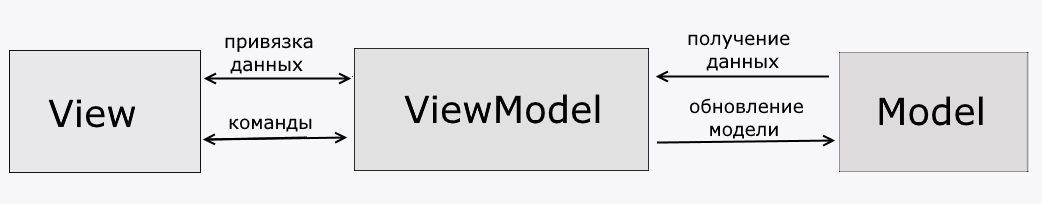
\includegraphics[scale=0.3]{mvvm.png} 
%    \caption{MVVM}
%    \label{fig:arch:docs_connections}
% \end{figure}

% Для упрощения реализации данной парадигмы проектирования и упрощения разработки, компания Google выпустила Android Architecture Components. Данный набор решений включает в себя:

% \begin{itemize}
%  \item Lifecycle - отслеживает текущий статус Activity и может уведомлять об этом своих подписчиков;
%  \item LiveData - получает и хранит данные, может отправлять их своим подписчикам;
%  \item ViewModel - поможет сохранить живыми необходимые для вас объекты при повороте экрана;
%  \item Paging Library - библиотека для постраничной загрузки данных из базы данных, с сервера или любого другого источника;
%  \item Navigation Architecture Component - новый компонент для навигации по экранам приложения;
%  \item Work Manager - удобный механизм выполнения фоновых задач;
%  \item Room - обёртка для работы с базой данных;
%  \item Data Binding - избавление от рутины по написанию кода работающего со View.
%  \end{itemize}

%  Основные плюсы MVVM включают в себя:

% \begin{itemize}
%   \item лёгкость в тестировании (связи между логикой приложения и пользовательским интерфейсом ослабевает, что даёт большую гибкость в тестировании отдельных компонентов);
%   \item прост в поддержке (высокая модульность и прозрачность слоёв архитектуры приносят простоту в отслеживании ошибок и расширении приложения);
%   \item прозрачная комьюникация (ViewModel предоставляют простой интерфейс, который View использует для заполнения себя, сама же ViewModel связывает View с частью бизнес-логики приложения).
% \end{itemize}
 
% \subsection{Serverless архитектура}
% Serverless-вычисления (бессерверные-вычисления) - модель облачных вычислений, в которых платформа динамически руководит выделением вычислительных ресурсов. 
% В данном случае бессерверный не означает отсутствие сервера как такового, под этим понимается то, что пользователю конкретной платформы не нужно заниматься созданием и настройкой собственного сервера. 
% Данный подход позволяет значительно сэкономить ресурсы и уменьшить срок разработки, так как многие важные аспекты серверной части на себе берёт платформа. 
% В рамках данного проекта такой платформой выступает Firebase.
 
% \subsection{Организация и описание модулей приложения}
% Разработанное мобильное приложение можно разделить на три составляющие:
% \begin{itemize}
%  \item Клиентское приложения на Kotlin;
%  \item Модуль Firebase для работы с базой данных;
%  \item API cервер для получения данных;
% \end{itemize}
 
% Клиентское приложение является основным модулем для данного проекта. В рамках клиентского приложения реализованы основные функциональные возможности данного проекта:
% \begin{itemize}
%   \item поддержка множества магазинов;
%   \item возможность фильтровать поиск по множеству фильтров;
%   \item вкладка избранное, возможность добавлять игры или предложения в избранное;
%   \item вкладка исследование, главная вкладка с предложениями которые ранжирует само приложение;
%   \item просмотр дополнительной информации (рейтинг, самая высокая стоимость, самая низкая стоимость и тд);
%   \item возможность перехода на сторонние магазины для покупки товара;
%   \item социальные функции (шейринг, отображение графики, ведение статистики пользователя).
% \end{itemize}
 
% Модуль Firebase отвечает за авторизацию, управление данными пользователя, их организацию и процесс передачи данных клиентскому приложению.
 
% API сервер представлет собой несколько API серверов с базами данных игр и игровых магазинов. Основная функция этих серверов заключается в выдаче клиенту необходимой для работы информации (список магазинов, дополнительная информация об игре, поиск лучший предложений).
 
% На рисунке~\ref{fig:arch:modules_scheme} изображена схема взаимодействия вышеперечисленных модулей.
 
% \begin{figure}[H]
%  \centering
%    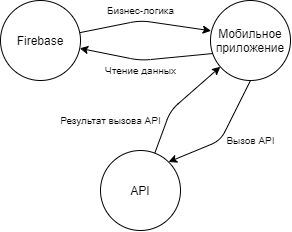
\includegraphics[scale=0.8]{api.png} 
%    \caption{Структура модулей приложения}
%    \label{fig:arch:modules_scheme}
% \end{figure}
 
% \section{Реализация мобильного приложения}
% \label{sec:code}
% По итогу разработки было реализовано мобильное приложение, которое позволяет пользователю находить лучшие предложения по продаже игр среди игровых магазинов. 